\section{Approach}
    \label{sec:1}
The general approach for answering the self-imposed question begins with processing the data according to the computational needs of the CNN and the hardware used. After that, an augmented data set of equally filled classes will be used to search for the CNN's optimal hyperparameters to avoid biases towards large populated classes. This optimized CNN will be trained on the original dataset with class imbalances and the augmented dataset to determine which of these datasets yields the highest precision in all classes. The best-performing dataset will undergo a cross-validation split and final training to produce precise and generalized results. In the following section, the data processing and architecture of the CNN will be presented in more detail.
\subsection{Data preprocessing}
The preprocessing of the data is a crucial step for the success of the chosen method. With the .jpg images being of size (360, 640) and the amount of data being high, down-scaling of the image's resolution and size becomes necessary for computational reasons. With this in mind, two methods were implemented, one doing a crop on the image to reduce the background, and the other one reducing the resolution of the image. 
The initial idea for the cropping was to use face detection software to dynamically crop each picture according to the driver's face position. This idea had to be dismissed as face detection was not as reliable as initially hoped. With many drivers in the "Distracted" class looking to the side or down on their phones, the face detection algorithm started to detect faces in the background of the images, introducing a large bias into the dataset. 
An alternative method was then chosen, which crops 100 pixels from the left and right of every picture, significantly reducing the amount of background for the training of the CNN. A before and after comparison of the cropped images can be seen in \autoref{fig:comp1}
\begin{figure}[H]
    \centering
    \begin{subfigure}{0.48\textwidth}
        \centering
        \adjustbox{valign=c}{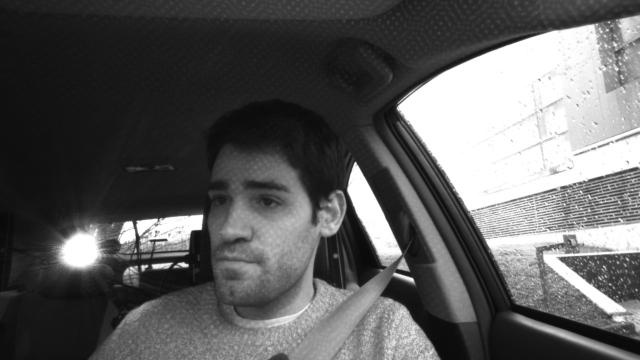
\includegraphics[width = \textwidth]{content/test1.jpg}}
    \end{subfigure}
    \hfill
    \begin{subfigure}{0.48\textwidth}
        \centering
        \adjustbox{valign=c}{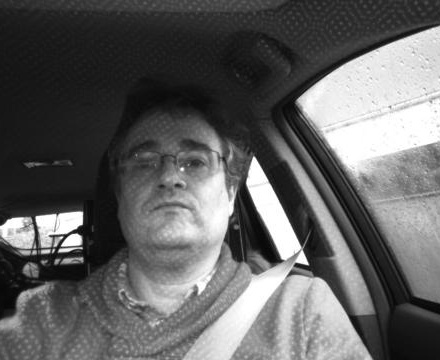
\includegraphics[width = \textwidth]{content/test2.jpg}}
    \end{subfigure}
    \caption{Comparison of the unprocessed (left) and processed (right) images.}
    \label{fig:comp1}
\end{figure}
\noindent
This hard cropping is possible due to the camera position being relatively consistent throughout all images. A larger crop sometimes led to the faces or class-relevant objects being cropped off and was thus dismissed. 
The cropped images were then scaled down to a resolution of 96 $\times$ 80 using the OpenCV \cite{opencv} library. A previous iteration of the CNN used 192$\times$160-pixel images which came with a large computational cost in the hyperparameter optimization and cross validation causing the software to crash. For that reason, the resolution had to be drastically decreased.
\subsection{Architecture of the model}
\label{sec:keinbockmehr}
The architecture of the model can be subdivided into convolutional and dense blocks, whose number of convolutional and dense layers respectively are obtained in the hyperparameter search. Max pooling is used in each convolutional block to increase feature extraction from the data and reduce its dimensionality, while each dense block contains a dropout layer to combat overfitting. The hyperparameter search was done using random search with a subsequent iterative Bayesian search algorithm on the constrained parameter space. The final architecture resulting from the hyperparameter search can be seen in \autoref{tab:arch}.
\begin{table}[H]
    \caption{The architecture of the neural network used for the final classification.}
    \vspace{0.2cm}
    \label{tab:arch}
    \centering
    \begin{adjustbox}{max width=\textwidth}
    \begin{tabular}{l|l|r}
        \toprule
        \multicolumn{3}{c}{\textbf{Architecture}} \\
        \midrule
        \textbf{Layer} & \textbf{Output Shape} & \textbf{Param \#} \\
        \midrule
 Input Layer & (None, 80, 96, 1) & 0 \\
 Conv2D & (None, 80, 96, 160) & 2,720 \\
 Conv2D & (None, 80, 96, 160) & 409,760 \\
 MaxPooling2D & (None, 40, 48, 160) & 0 \\
 Conv2D & (None, 40, 48, 160) & 409,760 \\
 Conv2D & (None, 40, 48, 160) & 409,760 \\
 MaxPooling2D & (None, 20, 24, 160) & 0 \\
 Conv2D & (None, 20, 24, 160) & 409,760 \\
 Conv2D & (None, 20, 24, 160) & 409,760 \\
 MaxPooling2D & (None, 10, 12, 160) & 0 \\
 Flatten & (None, 19200) & 0 \\
 Dense & (None, 448) & 8,602,048 \\
 Dropout & (None, 448) & 0 \\
 Dense & (None, 448) & 201,152 \\
 Dropout & (None, 448) & 0 \\
 Dense (Output) & (None, 6) & 2,694 \\
        \midrule
        \multicolumn{2}{l|}{\textbf{Total params}} & 10,857,414 \\
        \bottomrule
    \end{tabular}
    \end{adjustbox}
\end{table}
\noindent
The model has a 2D input shape of 96 $\times$ 80, resembling the final chosen size of the images. The CNN consists of 3 convolutional blocks followed by a flattening layer and 2 dense blocks with 448 dense units, based on the hyperparameter search. The max pooling size is 2 $\times$ 2 and the dropout rate is 0.5. Additional hyperparameters not directly related to the model's architecture are found in \autoref{tab:params}. A more detailed description of the search is found in Lennart's report.
\begin{table}[H]
    \caption{Additional hyperparameters and best Values.}
    \vspace{0.2cm}
    \label{tab:params}
    \centering
    \begin{adjustbox}{max width=\textwidth}
    \begin{tabular}{l|r}
        \toprule
        \textbf{Hyperparameter}  & \textbf{Final Value} \\
        \midrule
        \textbf{filters} & 160 \\
        \textbf{kernel\_size}  & 4 \\
        \textbf{regularizer\_strength}  & 0.06 \\
        \textbf{conv\_activation}  & elu \\
        \textbf{dense\_activation} & elu \\
        \textbf{learning\_rate} & 0.00011 \\
        \bottomrule
    \end{tabular}
    \end{adjustbox}
\end{table}
\noindent
The loss function chosen for the CNN is the categorical cross-entropy with an additional L2 regularization term. Precision will be the primary metric used, as it takes into account individual class performances which is of great importance when dealing with imbalanced classes.
The CNN's architecture is optimized for feature extraction with a large number of convolutional layers and is quite complex with a total of 10.857.414 trainable parameters. Additionally, an earlier unoptimized CNN will be used for comparisons consisting of 2 convolutional blocks of three convolutional layers and otherwise the same architecture with unoptimized hyperparameters. The input shape of the earlier model is 192$\times$160-pixel images due to it not being used in hyperparameter optimization or cross-validation.
\section{Data augmentation and overfitting optimization}
    \label{sec:2}
This section will present the precautions taken to compensate for possible overfitting of the data and the data augmentation done to balance the amount of classes in the dataset.
\subsection{Data augmentation}
Classes like "Yawn" or "Drinking" have very few entries in contrast to the rest of the dataset, with relative amounts to the total dataset size being 
Safe driving: 41.59\%,
Dangerous driving: 31.25\%,
Distracted: 14.00\%,
Sleepy driving: 6.59\%,
Yawn: 3.68\%,
Drinking: 2.89\% .
For this reason, data augmentation is implemented to account for these drastic class imbalances.
The approach chosen for the augmentation is to find a middle ground between balanced classes and computational cost due to the dataset's size. For this reason, every class is scaled to a total of 2000 images, with the largest three classes being cut, while the smallest three classes had to be filled with augmented images. 
The augmentation was conducted using the TensorFlow.keras.preprocessing.image.ImageDataGenerator method, alongside a self-implemented noise generator. The ImageDataGenerator does a random augmentation for each image based on initially set parameters. The augmentations applied to the images are shifts in width and height up to a value of 0.1, shear and zoom up to a value of 0.3 and 0.1 respectively, and a randomly set vertical flip. The noise generator applies random Gaussian noise to each pixel, with the strength of the noise being random for each image.
\begin{figure}[H]
    \centering
    \begin{subfigure}{0.48\textwidth}
        \centering
        \adjustbox{valign=c}{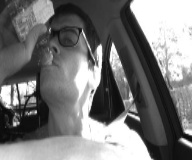
\includegraphics[width = \textwidth]{content/test_aug_1.jpg}}
    \end{subfigure}
    \hfill
    \begin{subfigure}{0.48\textwidth}
        \centering
        \adjustbox{valign=c}{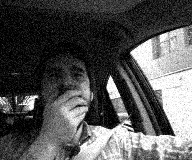
\includegraphics[width = \textwidth]{content/test_aug_2.jpg}}
    \end{subfigure}
    \caption{Two exemplary augmented pictures with zoom and shear (right) and noise (left).}
    \label{fig:comp2}
\end{figure}
\noindent
The augmentation method is randomly chosen for each image resulting in the augmentated images being roughly 50\% distorted and 50\% noisy. A total of 4047 augmented images were generated this way, while 6902 images were cut from the largest classes. 
Two exemplary augmented pictures can be seen in \autoref{fig:comp2}. The final CNN with optimized hyperparameters was then trained on both the original dataset and the augmented dataset with 2000 entries in each class. The confusion matrices for the training on both datasets can be seen in \autoref{fig:comp3}. 
\begin{figure}[H]
    \centering
    \begin{subfigure}{0.49\textwidth}
        \centering
        \adjustbox{valign=c}{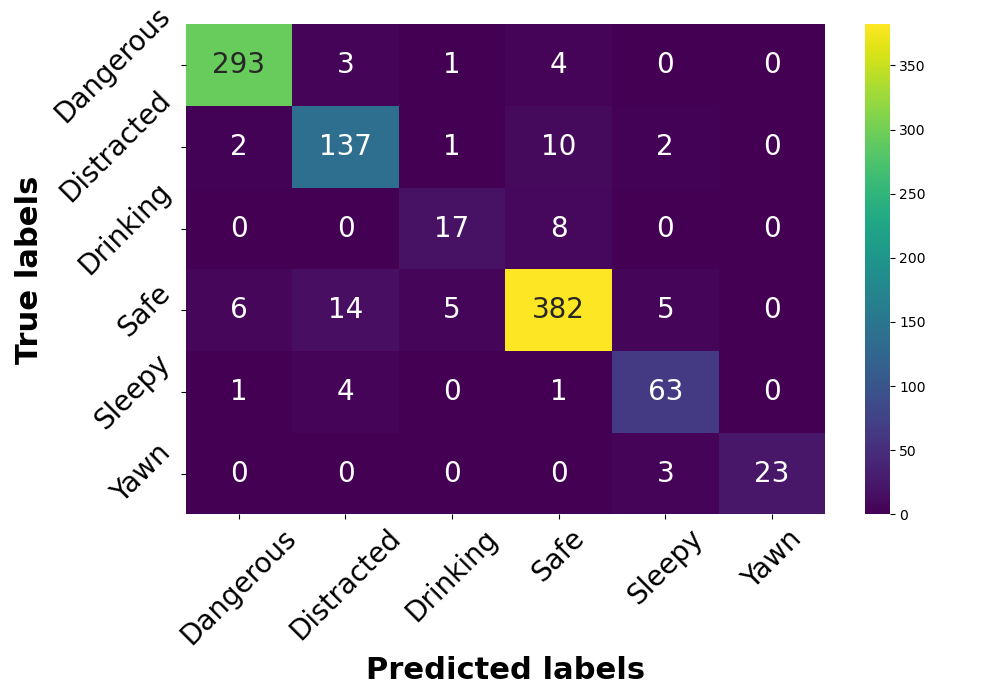
\includegraphics[width = \textwidth]{content/confusion_matrix_final_og.png}}
    \end{subfigure}
    \hfill
    \begin{subfigure}{0.49\textwidth}
        \centering
        \adjustbox{valign=c}{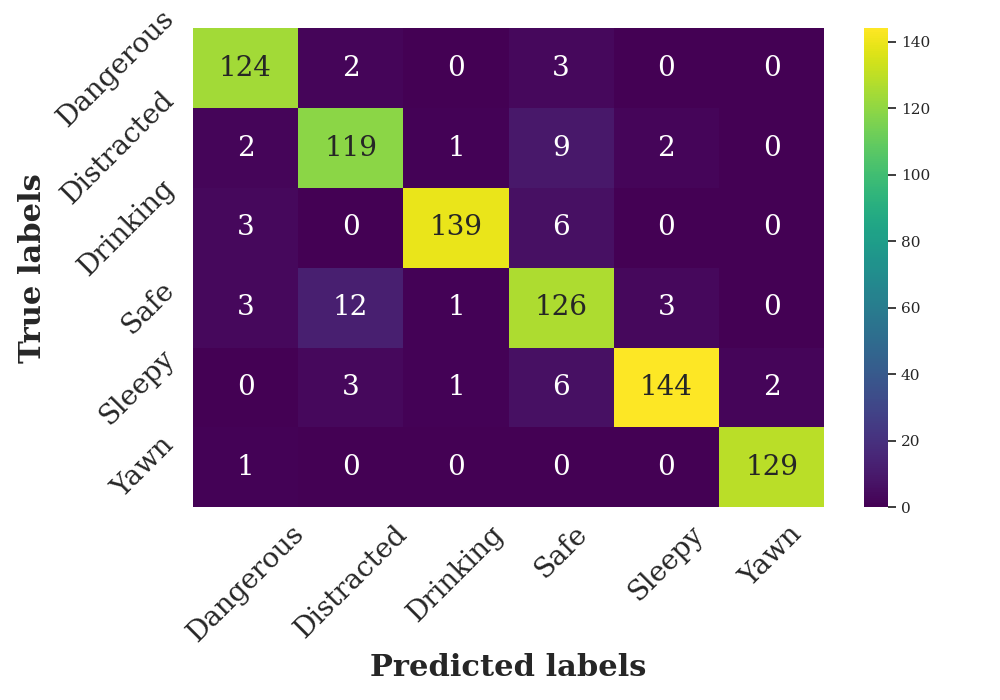
\includegraphics[width = \textwidth]{content/confusion_matrix_final_aug.png}}
    \end{subfigure}
    \caption{Confusion Matrices on the test data of the original dataset (left) and the augmented dataset (right).}
    \label{fig:comp3}
\end{figure}
\noindent
While most images are mostly classified correctly by both models, the confusion matrices in \autoref{fig:comp3} show the necessity of equally sized classes.
The left confusion matrix of the original dataset shows a great amount of misclassification of pictures labeled "Drinking". This is not only due to an inaccurate prediction but also due to the small number of entries labeled "Drinking" in the original test data, with a total of only 25 "Drinking" images. This shows a significantly decreased sensitivity in the low number of entry classes in comparison to the confusion matrix of the augmented dataset. For these reasons, the augmented dataset was chosen to undergo a final 12-fold cross-validation training to yield precise and generalized final results. The original dataset will still be used for a direct comparison to the alternative model as the alternative method is trained on imbalanced classes.
\subsection{Overfitting optimization}
To avoid overfitting, several methods were implemented, which will be explained in the following. The model itself contains 2 dropout layers, one in each dense block, with a dropout rate of 0.5. These layers reduce overfitting as dropping out random neurons during the training process increases the generalization of the model, thus reducing overfitting effects. Overfitting is further compensated for in the CNN by applying an L2 regularization, of regularization strength $\lambda = 0.06$, to the loss function. This regularization penalizes large weights, leading to a reduction of the model's complexity, which can be a reason for bad performance on unseen data.
The L2 regularization works by adding a term to the loss function which is then given by $$J(\theta) = \frac{1}{m} \sum_{i=1}^{m} L(y^{(i)}, h_\theta(x^{(i)})) + \frac{\lambda}{2m} \|\theta\|^2 \, .$$ The first term of the regularized loss function $J$ describes the traditional loss defined by the true label $y^{\left(i\right)}$ and the model prediction $h_\theta\left(x^{\left(i\right)}\right)$ while the second term describes the regularization proportional to the squared sum of weights $\|\theta\|^2$, penalizing huge weights. Both the dropout rate and regularization strength are hyperparameters, whose optimal values are obtained in the hyperparameter optimization.
\begin{figure}[H]
    \centering
    \begin{subfigure}{0.49\textwidth}
        \centering
        \adjustbox{valign=c}{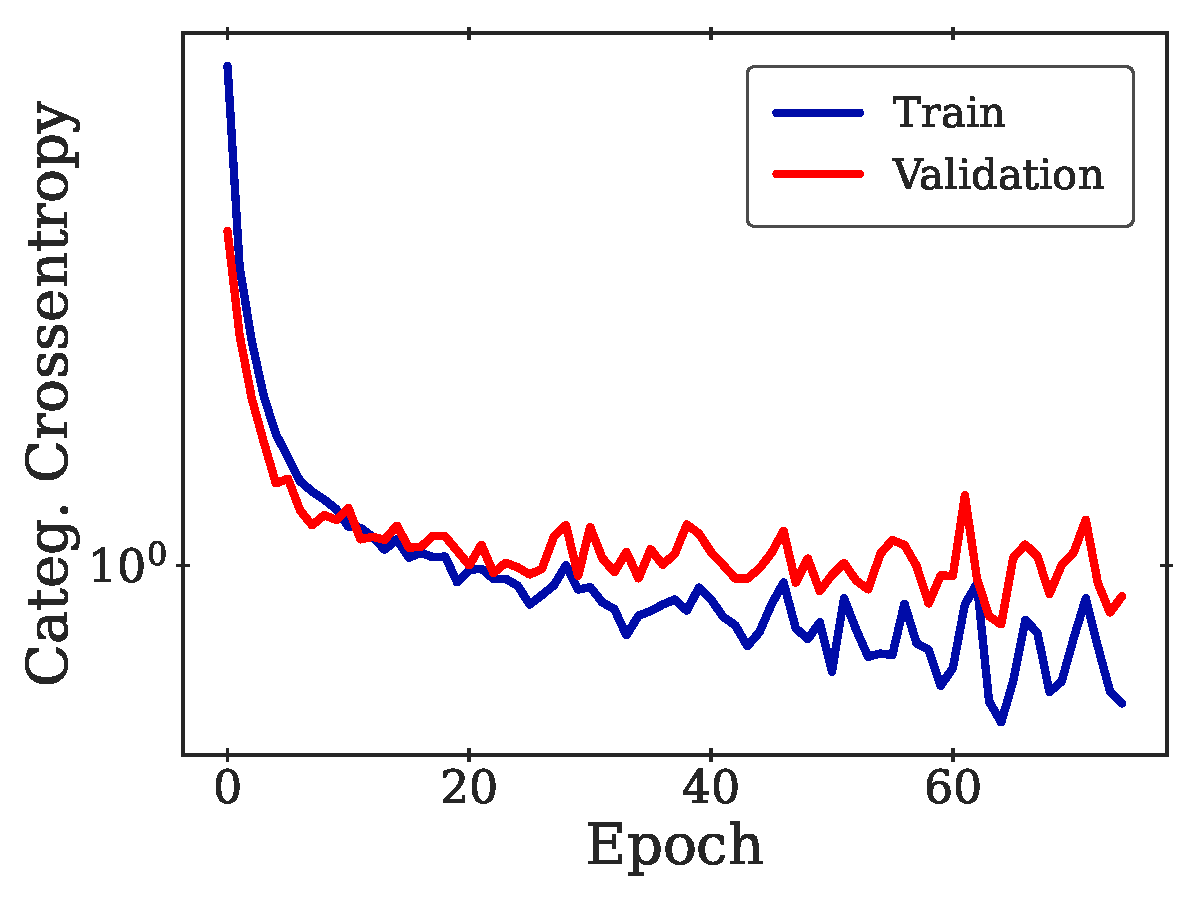
\includegraphics[width = \textwidth]{content/loss_bef_hyp.pdf}}
        \caption{Nonoptimal parameters without cross-validation, training performed on 192 $\times$ 160 images.}
    \end{subfigure}
    \hfill
    \begin{subfigure}{0.49\textwidth}
        \centering
        \adjustbox{valign=c}{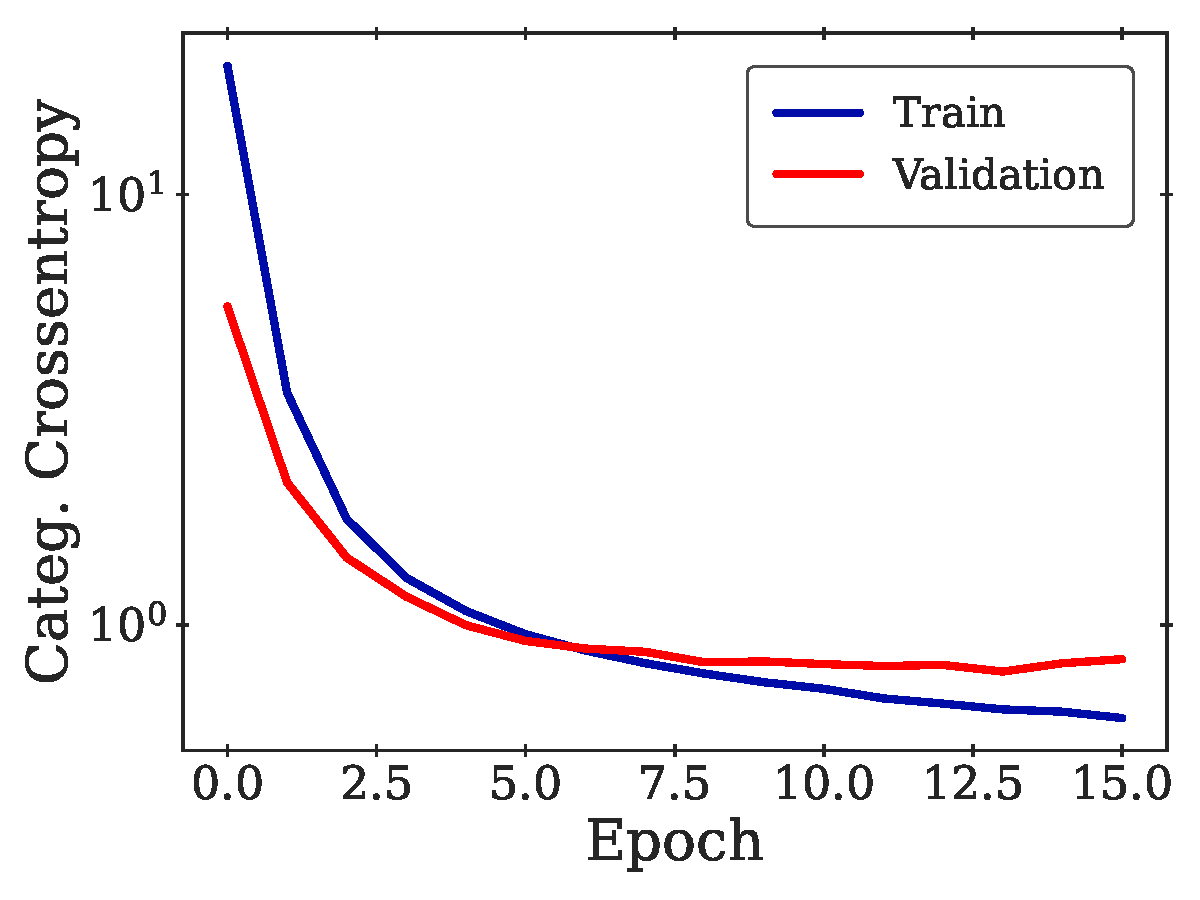
\includegraphics[width = \textwidth]{content/loss.pdf}}
        \caption{12-fold cross-validated loss with optimal parameters, training on 96 $\times$ 80 images.}
        \label{fig:comp4b}
    \end{subfigure}
    \caption{Effects of the optimized hyperparameters on overfitting.}
    \label{fig:comp4}
\end{figure}
\noindent
\autoref{fig:comp4} shows the loss per epoch before and after the hyperparameter optimization on the augmented data. Here the unoptimized model is the one described in \autoref{sec:keinbockmehr} using a significantly higher input resolution, while the plot on the right comes from the final training using a 12-fold cross-validation. Without optimized parameters in these regularization methods, the loss on the left shows clear signs of overfitting and large oscillations. While the optimized loss on the right shows a much better result, it still runs into overfitting issues. This is due to the limited size of the augmented dataset chosen, with a larger dataset having too much computational cost. A larger dataset with increased input image resolution would not run into overfitting as fast but would result in crashes on the used hardware or have to be aborted for time reasons. To combat the still-existing overfitting, early stopping was implemented, which sets the CNN's weights to the optimal values of a previous epoch, once a stagnation in the validation loss is detected. The patience of the early stopping is set to 5, to avoid a too early stopping of the training process. The effects of the early stopping can be seen in \autoref{fig:comp4}, as the training in the right plot is stopped much earlier due to a clearer stagnation of the validation loss. This prevents the usage of an overfit model even though overfitting may still occur during the final training process.
Additionally, a 12-fold cross-validation was implemented during the final training process to further validate the generalization of the model. The 12-fold cross-validation check was chosen to ensure that the model performs well on unseen data without sacrificing too much performance due to the limited size of the training sets. 
\section{Results and comparison to alternative Method}
    \label{sec:3}
    \subsection{Performance comparison to the Roboflow inference model}
The Roboflow inference model serving as the alternative method in this report is a pre-trained model using the Roboflow object detection platform (cite). The Roboflow model is trained on the same dataset provided on the Roboflow website in its original form \cite{rob_set}, which is why a comparison will be made on the unbalanced original test data to avoid biases in the Roboflow model. For this purpose the optimized CNN is trained on the processed training and validation data, provided by the original dataset, and evaluated on the processed test data to be comparable with the Roboflow model evaluated on the unprocessed test data. 
The metrics of both models can be seen in \autoref{tab:comp_rob}
\begin{table}[H]
    \centering
    \caption{Performance comparison between the Roboflow model including and excluding unidentified images and the self-trained CNN.}
    \vspace{3pt}
    \label{tab:comp_rob}
    \begin{adjustbox}{max width=\textwidth}
    \begin{tabular}{l|cc|c|cc|c|cc|c}
        \toprule
        \textbf{Class} & \multicolumn{3}{c|}{\textbf{Roboflow, excl. unidentified}} & \multicolumn{3}{c|}{\textbf{Roboflow, incl. unidentified}} & \multicolumn{3}{c}{\textbf{CNN}} \\
        \cmidrule{2-10}
         & \textbf{Precision} & \textbf{Recall} & \textbf{Entries} & \textbf{Precision} & \textbf{Recall} & \textbf{Entries} & \textbf{Precision} & \textbf{Recall} & \textbf{Entries} \\
        \midrule
 Dangerous & 0.98 & 0.99 & 274 & 0.98 & 0.90 & 301 & 0.97 & 0.97 & 301 \\
 Distracted & 0.95 & 0.84 & 118 & 0.95 & 0.65 & 152 & 0.87 & 0.90 & 152 \\
 Drinking & 0.95 & 1.00 & 18 & 0.95 & 0.72 & 25 & 0.71 & 0.68 & 25 \\
 Safe & 0.94 & 0.96 & 331 & 0.94 & 0.77 & 412 & 0.94 & 0.93 & 412 \\
 Sleepy & 1.00 & 0.87 & 45 & 1.00 & 0.57 & 69 & 0.86 & 0.91 & 69 \\
 Yawn & 0.69 & 1.00 & 25 & 0.69 & 0.96 & 26 & 1.00 & 0.88 & 26 \\
        \midrule
 Macro avg & 0.92 & 0.94 & 811 & 0.79 & 0.65 & 985 & 0.89 & 0.88 & 985 \\
 Accuracy & 0.95 & \phantom{0} & 811 & 0.78 & \phantom{0} & 985 & 0.93 & \phantom{0} & 985 \\
        \bottomrule
    \end{tabular}
    \end{adjustbox}
\end{table}
\noindent 
The Roboflow model, accessed via the Roboflow API (cite), sometimes fails to classify a given image for unknown reasons. This results in better metrics when unidentified images are excluded from the evaluation, as portrayed in the left three columns of \autoref{tab:comp_rob}. For comparability the unidentified cases were included in the middle three columns of \autoref{tab:comp_rob} which results in much worse metrics on the test data for the Roboflow model, being outperformed by the CNN in the average metrics and accuracy. 
The confusion matrices shown in \autoref{fig:conf_comp} compare the results obtained by the CNN and the results of the Roboflow model when not excluding the unidentified images, represented by the extra column.
\begin{figure}[H]
    \centering
    \begin{subfigure}{0.49\textwidth}
        \centering
        \adjustbox{valign=c}{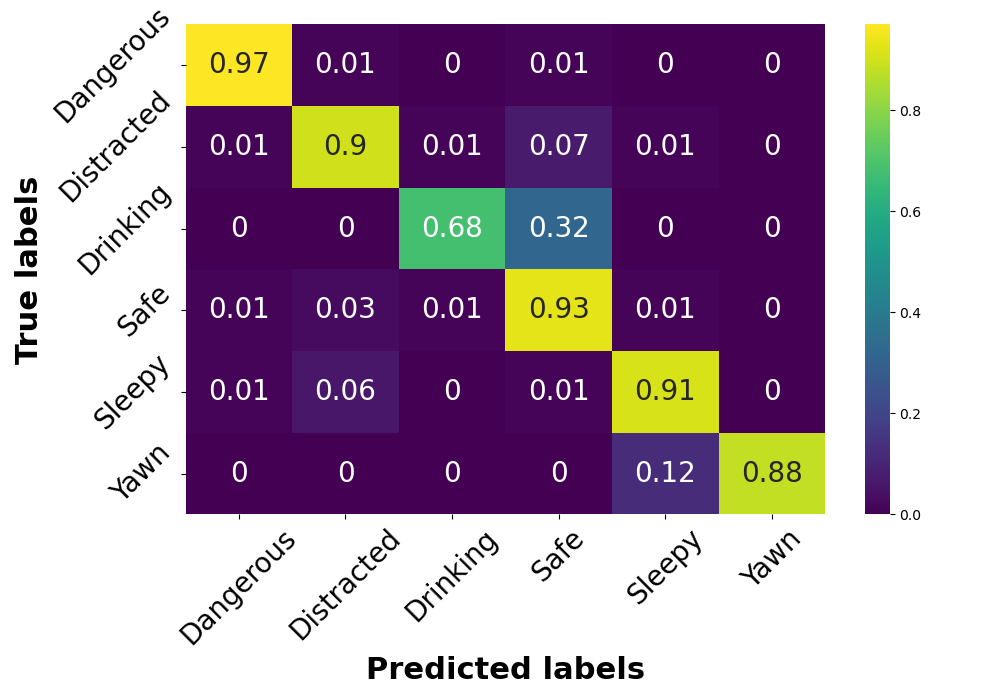
\includegraphics[width = \textwidth]{content/confusion_matrix_final_og_norm.png}}
        \caption{Confusion matrix of CNN on processed original test data.}
    \end{subfigure}
    \hfill
    \begin{subfigure}{0.49\textwidth}
        \centering
        \adjustbox{valign=c}{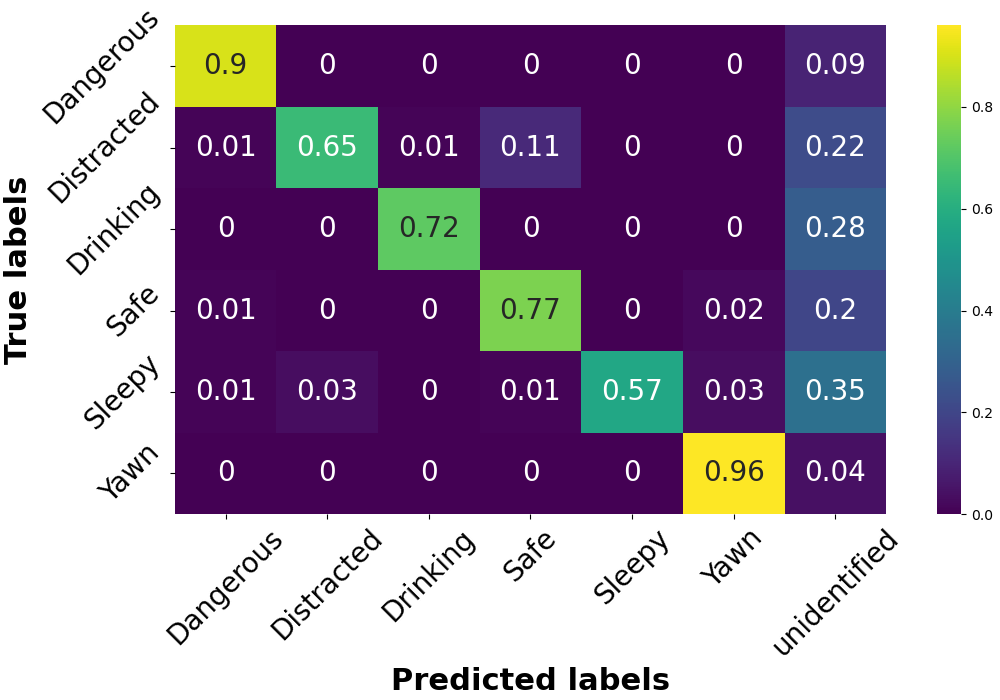
\includegraphics[width = \textwidth]{content/confusion_matrix_robo_unid.png}}
        \caption{Confusion matrix of Roboflow model on original test data, including unidentified images.}
    \end{subfigure}
    \caption{Comparison of the confusion matrices.}
    \label{fig:conf_comp}
\end{figure}
\noindent
The rows of the matrices in \autoref{fig:conf_comp} have been normalized for visibility reasons due to the class imbalances, portraying each class's recall on the diagonal.
This comparison shows a much better performance of the CNN compared to the Roboflow model, even though the CNN's classification still lacks sensitivity in the low-entry classes on the original imbalanced test data. 
\subsection{Final performance of the CNN}
The CNN's performance is evaluated on a 12-fold cross-validation dataset as described in the previous section and the results are averaged across all folds. With the optimal parameters obtained in the hyperparameter optimization and training on the augmented dataset of equally sized classes, the maximum performance achievable by the CNN in this report can be seen in \autoref{tab:perf}.
\begin{table}[H]
    \centering
    \caption{Classification Report for Model}
    \vspace{3pt}
    \label{tab:perf}
    \begin{adjustbox}{max width=\textwidth}
    \begin{tabular}{l|cc|c}
        \toprule
        \textbf{Class} & \textbf{Precision} & \textbf{Recall} & \textbf{Entries} \\
        \midrule
 Dangerous & 0.96 & 0.94 & 2003 \\
 Distracted & 0.87 & 0.88 & 2000 \\
 Drinking & 0.94 & 0.96 & 1998 \\
 Safe & 0.85 & 0.84 & 2000 \\
 Sleepy & 0.89 & 0.90 & 2000 \\
 Yawn & 0.94 & 0.95 & 1999 \\
        \midrule
 Macro avg & 0.91 & 0.91& 12000 \\
 Accuracy & 0.91 & \phantom{0} & 12000 \\
        \bottomrule
    \end{tabular}
    \end{adjustbox}
\end{table}
\noindent
With an average precision and recall of 91\% the CNN performs very well on the balanced classes. The lowest metrics are in the "Distracted" and "Safe" classes with "only" 87\% and 85\% respectively. This is likely due to a relatively high confusion in these two classes as can be seen in this model's confusion matrix in \autoref{fig:conf_fin}
\begin{figure}[H]
    \centering
    \begin{subfigure}{0.49\textwidth}
        \centering
        \adjustbox{valign=c}{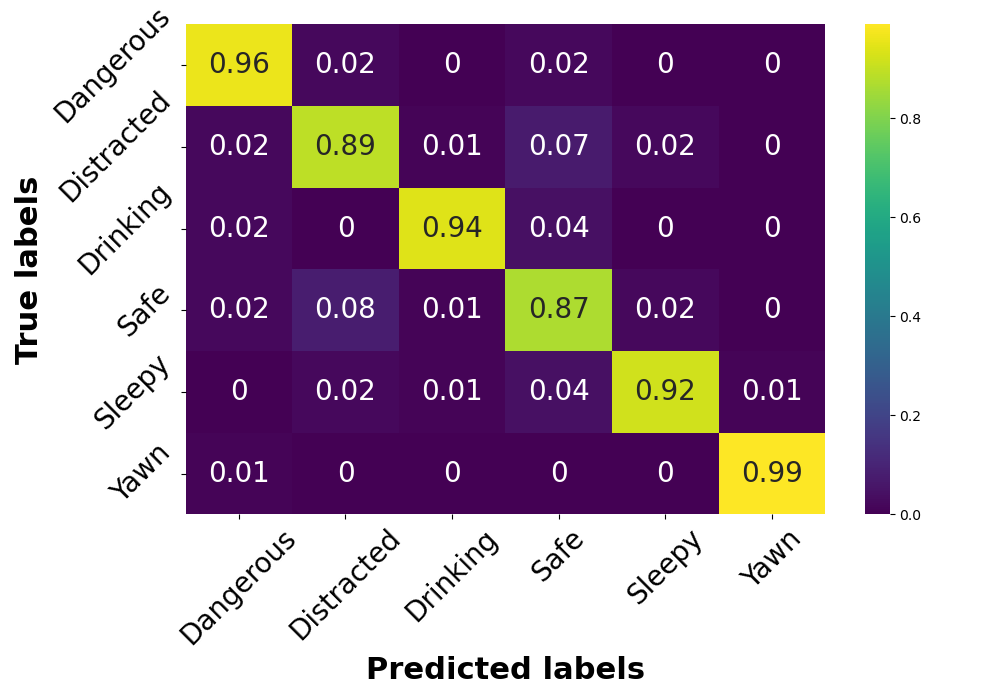
\includegraphics[width = \textwidth]{content/confusion_matrix_final_aug_norm.png}}
        \caption{Confusion matrix of CNN on 12-fold cross-validated augmented dataset.}
        \label{fig:conf_fin}
    \end{subfigure}
    \hfill
    \begin{subfigure}{0.49\textwidth}
        \centering
        \adjustbox{valign=c}{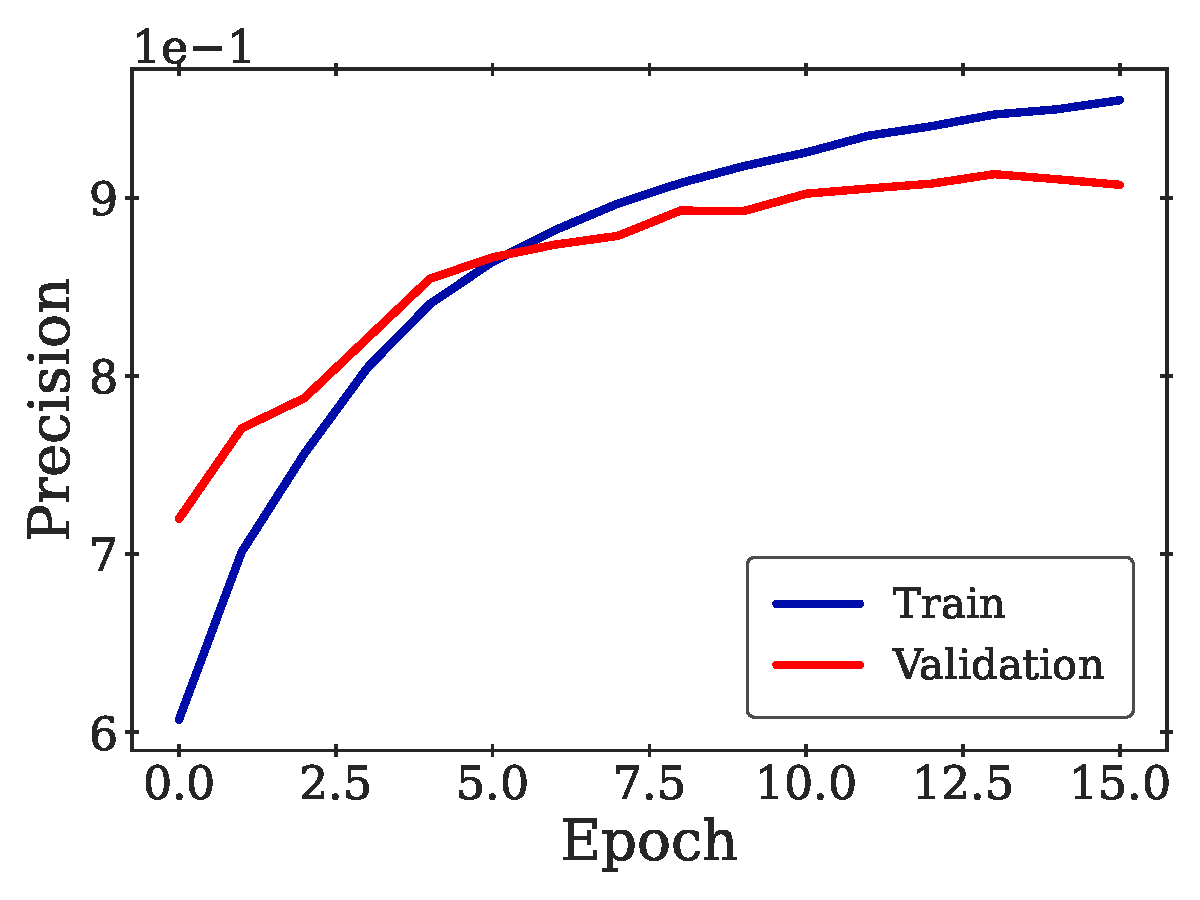
\includegraphics[width = \textwidth]{content/prec.pdf}}
        \caption{Precision per epoch of CNN on the 12-fold cross-validated augmented dataset.}
        \label{fig:prec}
    \end{subfigure}
\end{figure}
\noindent
With a high reduction of the data by downscaling it to a resolution of 96 $\times$ 80 for the cross-validation and hyperparameter search, small details like looking direction in the eyes, get lost. The classes "Safe" and "Distraced" are distinguished by such small details with "Distraced" drivers often looking to the side or down on their phone. A relatively "high" confusion is thus to be expected. 
\autoref{fig:prec} shows the average precision per epoch during the training on the augmented dataset. While this graph shows some overfitting, this is due to the limited amount and resolution and number of entries of the data as described in the previous section and does not cause a nongeneralization of the presented results as the early stopping prevents actual overfitting of the CNN.
